\documentclass[]{article}
\usepackage{lmodern}
\usepackage{amssymb,amsmath}
\usepackage{ifxetex,ifluatex}
\usepackage{fixltx2e} % provides \textsubscript
\ifnum 0\ifxetex 1\fi\ifluatex 1\fi=0 % if pdftex
  \usepackage[T1]{fontenc}
  \usepackage[utf8]{inputenc}
\else % if luatex or xelatex
  \ifxetex
    \usepackage{mathspec}
  \else
    \usepackage{fontspec}
  \fi
  \defaultfontfeatures{Ligatures=TeX,Scale=MatchLowercase}
\fi
% use upquote if available, for straight quotes in verbatim environments
\IfFileExists{upquote.sty}{\usepackage{upquote}}{}
% use microtype if available
\IfFileExists{microtype.sty}{%
\usepackage{microtype}
\UseMicrotypeSet[protrusion]{basicmath} % disable protrusion for tt fonts
}{}
\usepackage[margin=1in]{geometry}
\usepackage{hyperref}
\hypersetup{unicode=true,
            pdftitle={Template manuscript},
            pdfauthor={Oscar de Grouche, Jane Doe},
            pdfborder={0 0 0},
            breaklinks=true}
\urlstyle{same}  % don't use monospace font for urls
\usepackage{graphicx,grffile}
\makeatletter
\def\maxwidth{\ifdim\Gin@nat@width>\linewidth\linewidth\else\Gin@nat@width\fi}
\def\maxheight{\ifdim\Gin@nat@height>\textheight\textheight\else\Gin@nat@height\fi}
\makeatother
% Scale images if necessary, so that they will not overflow the page
% margins by default, and it is still possible to overwrite the defaults
% using explicit options in \includegraphics[width, height, ...]{}
\setkeys{Gin}{width=\maxwidth,height=\maxheight,keepaspectratio}
\IfFileExists{parskip.sty}{%
\usepackage{parskip}
}{% else
\setlength{\parindent}{0pt}
\setlength{\parskip}{6pt plus 2pt minus 1pt}
}
\setlength{\emergencystretch}{3em}  % prevent overfull lines
\providecommand{\tightlist}{%
  \setlength{\itemsep}{0pt}\setlength{\parskip}{0pt}}
\setcounter{secnumdepth}{0}
% Redefines (sub)paragraphs to behave more like sections
\ifx\paragraph\undefined\else
\let\oldparagraph\paragraph
\renewcommand{\paragraph}[1]{\oldparagraph{#1}\mbox{}}
\fi
\ifx\subparagraph\undefined\else
\let\oldsubparagraph\subparagraph
\renewcommand{\subparagraph}[1]{\oldsubparagraph{#1}\mbox{}}
\fi

%%% Use protect on footnotes to avoid problems with footnotes in titles
\let\rmarkdownfootnote\footnote%
\def\footnote{\protect\rmarkdownfootnote}

%%% Change title format to be more compact
\usepackage{titling}

% Create subtitle command for use in maketitle
\newcommand{\subtitle}[1]{
  \posttitle{
    \begin{center}\large#1\end{center}
    }
}

\setlength{\droptitle}{-2em}
  \title{Template manuscript}
  \pretitle{\vspace{\droptitle}\centering\huge}
  \posttitle{\par}
  \author{Oscar de Grouche, Jane Doe}
  \preauthor{\centering\large\emph}
  \postauthor{\par}
  \predate{\centering\large\emph}
  \postdate{\par}
  \date{April 15, 2017}


\begin{document}
\maketitle

\section{Abstract}\label{abstract}

Abstract text would go here.

\section{Introduction}\label{introduction}

This is an R Markdown document. Markdown is a simple formatting syntax
for authoring HTML, PDF, and MS Word documents. For more details on
using R Markdown see \url{http://rmarkdown.rstudio.com}.

When you click the \textbf{Knit} button a document will be generated
that includes both content as well as the output of any embedded R code
chunks within the document. You can \textbf{Knit} to PDF or to Microsoft
word, just chose the appropriate dropdown from the \textbf{Knit} button.

\section{Methods}\label{methods}

You can make words \textbf{bold} with two asterisks, \emph{italicized}
with one.

\subsection{Data}\label{data}

Hashtags denote a header, and the hierarchy is defined by the number of
hashtags.

\subsection{Statistical Analysis}\label{statistical-analysis}

To make a floating equation, use two dollar signs on either side:

\[
\text{logit}(g_l) = \beta_{0g} + \beta_{1g}x_l.
\]

To make an in-line equation, use one dollar sign. As in this:
\(\alpha_\gamma^2\) for an example.

To make an equation array that shows up in both Word and PDF, you can
use the following format:

\[
\begin{aligned}
R  &=  \text{the number of sightability trials (here }R = 124)\\
z_l &= \text{a random variable equal to 1 when the }l\text{th group is detected and 0 otherwise } (l = 1,2, \ldots, R)\\
x_l &= \text{the percent visual obstruction (from 0 to 1) associated with the }l\text{th group } (l = 1,2, \ldots, R)\\
g_l &= \text{the probability of detection of the }l\text{th group } (l = 1,2, \ldots, R)
\end{aligned}
\]

Remember to put ampersands (\&) to align equations.

\section{Results}\label{results}

\subsection{Results sub-section}\label{results-sub-section}

\section{Discussion}\label{discussion}

You can cite references using the \textbf{citr} add-in. With
\textbf{citr} you can cite papers in line like Fieberg and Guidice
(2008) is fond of doing, or parenthetically (R Development Core Team
2014). You can also cite multiple sources at once (Fieberg and Guidice
2008, Plummer 2013, Buckland et al. 2015). References can be added into
the myrefs.bib file directly, or created with BibTeX through LaTeX.

\section{Figures}\label{figures}

Figures can be included with the following code, but they must be in
.png format to show up in both Word and PDF. They can be referenced for
the PDF with Fig. \ref{figure1}. \emph{Unfortunately, I don't yet know
how to make the reference number show up in Word.}

\begin{figure}[htbp]
\centering
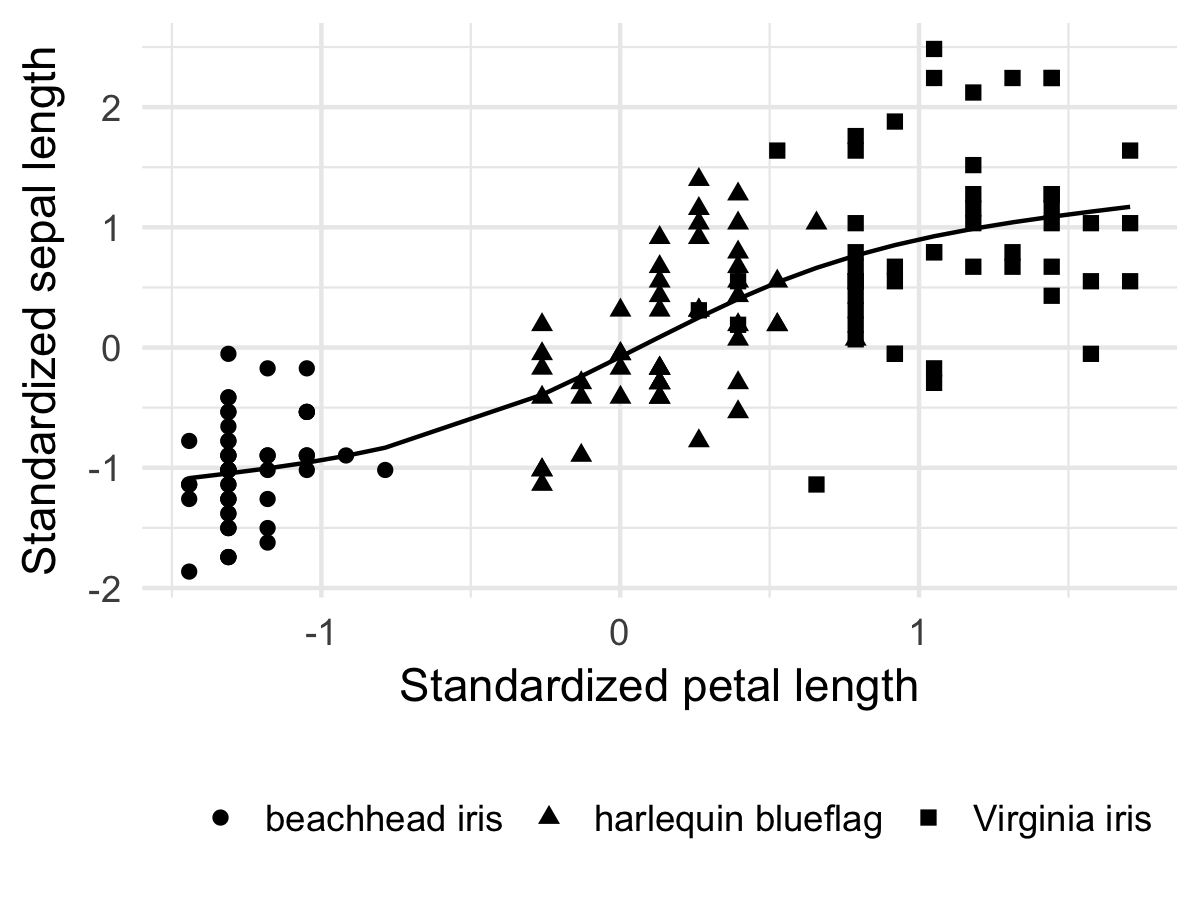
\includegraphics{ms_figures/figure1.png}
\caption{1. Example figure caption, which can include in-line equations
like \(y = \alpha + \beta x\) and references like Fieberg and Guidice
(2008). \label{figure1}}
\end{figure}

\section*{References}\label{references}
\addcontentsline{toc}{section}{References}

\hypertarget{refs}{}
\hypertarget{ref-Buckland:2015}{}
Buckland, S. T., E. A. Rexstad, T. A. Marques, and C. S. Oedekoven.
2015. Distance Sampling: Methods and Applications. Springer,
Switzerland.

\hypertarget{ref-Fieberg:2008}{}
Fieberg, J. R., and J. H. Guidice. 2008. Variance of stratified survey
estimators with probability of detection estimates. The Journal of
Wildlife Management 72:837--844.

\hypertarget{ref-Plummer:2013}{}
Plummer, M. 2013. JAGS Version 3.4.0 user manual.

\hypertarget{ref-R:2014}{}
R Development Core Team. 2014. R: A Language and Environment for
Statistical Computing. R Foundation for Statistical Computing, Vienna,
Austria.


\end{document}
